% !TeX encoding = UTF-8

%% ------------------------------------------------------------------------
%% Copyright (C) 2021-2023 SJTUG
%% 
%% SJTUBeamer Example Document by SJTUG
%% 
%% SJTUBeamer Example Document is licensed under a
%% Creative Commons Attribution-NonCommercial-ShareAlike 4.0 International License.
%% 
%% You should have received a copy of the license along with this
%% work. If not, see <http://creativecommons.org/licenses/by-nc-sa/4.0/>.
%%
%% For a quick start, check out src/doc/sjtubeamerquickstart.tex
%% Join discussions: https://github.com/sjtug/SJTUBeamer/discussions
%% -----------------------------------------------------------------------

\documentclass[xcolor=table,dvipsnames,svgnames,aspectratio=169]{ctexbeamer}
% 可以通过 fontset=macnew / fontset=ubuntu / fontset=windows 选项切换字体集；
% 如遇无法显示的数学符号，尝试对 ctexbeamer 文档类添加 no-math 选项；
% 写纯英文幻灯片可以改用 beamer 文档类。

\usepackage{tikz}
\usepackage[normalem]{ulem}
\usetikzlibrary{arrows}
\usepackage{amsmath}
\usepackage{graphicx}
\usepackage{hologo}
\usepackage{colortbl}
\usepackage{shapepar}
\usepackage{hyperxmp}
\usepackage{booktabs}
\usepackage{listings}
\usepackage{tipa}
\usepackage{multicol}
\usepackage{datetime2}
\usepackage{fontawesome5}
\usepackage{hyperref}

% 参考文献设置，使用 style=gb7714-2015 样式为标准顺序编码制，
% 使用 style=gb7714-2015ay 样式可以改为著者-出版年制。
\usepackage[backend=biber,style=gb7714-2015]{biblatex}
\addbibresource{ref.bib}

\graphicspath{{figures/}}

\hypersetup{
  pdfcopyright = {Licensed under CC-BY-SA 4.0. Some rights reserved.},
  pdflicenseurl = {http://creativecommons.org/licenses/by-sa/4.0/},
  unicode = true,
  psdextra = true,
  pdfdisplaydoctitle = true
}

\pdfstringdefDisableCommands{
  \let\\\relax
  \let\quad\relax
  \let\hspace\@gobble
}

\renewcommand{\TeX}{\hologo{TeX}}
\renewcommand{\LaTeX}{\hologo{LaTeX}}
\newcommand{\BibTeX}{\hologo{BibTeX}}
\newcommand{\XeTeX}{\hologo{XeTeX}}
\newcommand{\pdfTeX}{\hologo{pdfTeX}}
\newcommand{\LuaTeX}{\hologo{LuaTeX}}
\newcommand{\MiKTeX}{\hologo{MiKTeX}}
\newcommand{\MacTeX}{Mac\hologo{TeX}}
\newcommand{\beamer}{\textsc{beamer}}
\newcommand{\XeLaTeX}{\hologo{Xe}\kern-.13em\LaTeX{}}
\newcommand{\pdfLaTeX}{pdf\LaTeX{}}
\newcommand{\LuaLaTeX}{Lua\LaTeX{}}

\def\TeXLive{\TeX{} Live}
\let\TL=\TeXLive
\newcommand{\SJTUThesis}{\textsc{SJTUThesis}}
\newcommand{\SJTUThesisVersion}{2.0.3}
\newcommand{\SJTUThesisDate}{2023/9/25}
\newcommand{\SJTUBeamer}{\textsc{SJTUBeamer}}
\newcommand{\SJTUBeamerVersion}{3.0.0}
\newcommand{\SJTUBeamerDate}{2022/11/22}

\newcommand\link[1]{\href{#1}{\faLink}}
\newcommand\pkg[1]{\texttt{#1}}

\def\cmd#1{\texttt{\color{structure}\footnotesize $\backslash$#1}}
\def\env#1{\texttt{\color{structure}\footnotesize #1}}
\def\cmdxmp#1#2#3{\small{\texttt{\color{structure}$\backslash$#1}\{#2\}
\hspace{1em}\\ $\Rightarrow$\hspace{1em} {#3}\par\vskip1em}}

\usetheme[maxplus]{sjtubeamer}
% 使用 maxplus/max/min 切换标题页样式
% 使用 red/blue 切换主色调
% 使用 light/dark 切换亮/暗色模式
% 使用外样式关键词以获得不同的边栏样式
%   miniframes infolines  sidebar
%   default    smoothbars split	 
%   shadow     tree       smoothtree
% 使用 topright/bottomright 切换徽标位置
% 使用逗号分隔列表以同时使用多种选项

% \setbeamertemplate{background}{}
% 对于 max 主题，如果需要关闭正文背景图，请取消注释上一行。

% \tikzexternalize[prefix=build/]
% 如果您需要缓存 tikz 图像，请取消注释上一行，并在编译选项中添加 -shell-escape。

\lstset{
  language=[LaTeX]TeX,           % 更改高亮语言
  texcsstyle=*\color{cprimary},  % 只在高亮 LaTeX 语言时必须
  tabsize=2,
  basicstyle=\ttfamily\small,%
  keywordstyle=\color{cprimary},%
  stringstyle=\color{csecondary},%
  commentstyle=\color{ctertiary!50!gray},%
  breaklines,%
}

\author{Nan LIN}
\institute[Nan LIN]{上海交通大学}
\date{\the\year 年 \the\month 月}
\subject{Physics}

%%% -------------------------
%%% 页脚标题和首页标题
\title[Introduction to Electrodynamics] % 页脚显示标题
{\textbf{电动力学导论}} % 首页标题

%%% 副标题
\subtitle{Introduction to Electrodynamics}
%%% ------------------------

\begin{document}

% 使用节目录
\AtBeginSection[]{
  \begin{frame}
    %% 使用传统节目录，也可以将 subsectionstyle=... 换成 hideallsubsections 以隐藏所有小节信息
    \tableofcontents[currentsection,subsectionstyle=show/show/hide]
    %% 或者使用节页
    % \sectionpage
  \end{frame}
}

% 使用小节目录
\AtBeginSubsection[]{		       % 在每小节开始
  \begin{frame}
    %% 使用传统小节目录
    \tableofcontents[currentsection,subsectionstyle=show/shaded/hide]
    %% 或者使用小节页
    % \subsectionpage
  \end{frame}
}

\maketitle

\section{Electric Fields in Matter} % (fold)
\label{sec:Electric Fields in Matter}

\subsection{Polarization} % (fold)
\label{sub:Polarization}

\begin{frame}
  \frametitle{Dielectrics}

  In most everday objects belong to one of two larges classes:
  \begin{itemize}

      \item \textbf{Conductors}: charges aree free to move about through the material, not associated twith any particular nucleus but roam around at will

      \item \textbf{Dielectrics (Insulators)}: All charges are attached to specific atoms or molecules, all they can do is move a bit within the atom or molecule.

  \end{itemize}

  Two principal mechanisms: Electric fields can distort the charge distribution of a dielectric atom or molecule: \textit{stretching} and \textit{rotating}.



\end{frame}

\begin{frame}
  \frametitle{Induced Dipoles}

  What happens to a neutral atom when it is placed in electric field $\overrightarrow{E}$ ?

  \begin{itemize}

      \item Although the atom as a whole is electrically neutral, there is a positively charged core (the nucleus) and a negatively charged electron.
      \item The nucleus is pushed in the direction of the field, and the electrons the opposite way.

  \end{itemize}

  The atom is \textbf{polarized}, with a tiny \textbf{dipole moment} $\overrightarrow{p}$, which points in the same direction as $\overrightarrow{E}$, proportional to the field:
  \begin{equation}
    \overrightarrow{p} = \alpha \overrightarrow{E}
  \end{equation}

  where $\alpha$ is called \textbf{atomic polarizability}.



\end{frame}

\begin{frame}
  \frametitle{Induced Dipoles}

  For some neutral molecules like carbon dioxide, they frequently polarize more readily in some directions than in others, for example:
  \begin{equation}
    \overrightarrow{p} = \alpha_\perp \overrightarrow{E}_\perp + \alpha_\parallel \overrightarrow{E}_\parallel
  \end{equation}

  For a completely asymmetrical molecule, there is the most general linear relationship between $\overrightarrow{E}$ and $\overrightarrow{p}$:
  \begin{equation}
    \begin{cases}
      p_x = \alpha _{xx} E_x + \alpha _{xy} E_y + \alpha_{xz} E_z \\
      p_y = \alpha _{yx} E_x + \alpha _{yy} E_y + \alpha_{zz} E_z \\
      p_z = \alpha _{zx} E_x + \alpha _{zy} E_y + \alpha_{zz} E_z 
    \end{cases}
  \end{equation}

  The induced dipole moment may not be in the same direction as $\overrightarrow{E}$.

\end{frame}

\begin{frame}
  \frametitle{Alignment of polar molecules}


  For some molecules which have built-in, permanent dipole moments, called \textbf{polar molecules}, e.g. water molecule, 
  \begin{itemize}

      \item If the champ is uniform, the force on the positive end exactly cancels the force on the negative end. However, there will be a torique
        \begin{align}
          \overrightarrow{N} &= \overrightarrow{F}_- \overrightarrow{r}_- + \overrightarrow{F}_+  \overrightarrow{r}_+ 
                             = \frac{\overrightarrow{d}}{2} \times q \overrightarrow{E} - \frac{\overrightarrow{d}}{2} \times (-q \overrightarrow{E}) = q \overrightarrow{d} \times \overrightarrow{E} \\
                             &= q \overrightarrow{d} \times \overrightarrow{E} = \overrightarrow{p} \times \overrightarrow{E} 
                            = \displaystyle\frac{1}{4 \pi \epsilon_0} 
        \end{align}




  \end{itemize}

\end{frame}

\begin{frame}
  \frametitle{Alignment of molecules and polar molecules}



  \begin{itemize}

      \item If the champ is not uniform, $\overrightarrow{F}_+$ does not balance $\overrightarrow{F}_+$, there will be a net force on the dipole:
        \begin{equation}
          \overrightarrow{F} = \overrightarrow{F}_+ + \overrightarrow{F}_- = q(\overrightarrow{E}_+ - \overrightarrow{E}_-) = q(\Delta \overrightarrow{E})
        \end{equation}

  Assuming the dipole is very short, we approximate the small change in the electric field:

  \begin{equation}
    \Delta E_x = \nabla E_x . \overrightarrow{d},\quad \Delta \overrightarrow{E} = (\overrightarrow{d}. \nabla) \overrightarrow{E}
  \end{equation}

  and therefore 
  \begin{equation}
    \overrightarrow{F} = (\overrightarrow{p}.\nabla)\overrightarrow{E}
  \end{equation}



  \end{itemize}

  The torque about the center of the dipole in a nonuniform field is:
  \begin{equation}
    \overrightarrow{N} = \overrightarrow{p} \times \overrightarrow{E} + \overrightarrow{r} \times \overrightarrow{F}
  \end{equation}

\end{frame}
\begin{frame}
  \frametitle{Polarization - Conclusion}

  The result of placing a piece of dielectric material in an electric field is that the material becomes \textbf{polarized}, i.e. pointing along the direction of the field, either a tiny dipole moment is induced for neutral atoms, or a torque for polar molecules.

  A measure for this effect is 
  \begin{equation}
    \overrightarrow{P} = \text{dipole moment per unit volume}
  \end{equation}

  which is called \textbf{polarization}.

\end{frame}
% subsection Polarization (end)

\subsection{The field of a polarized object} % (fold)
\label{sub:The field of a polarized object}

\begin{frame}
  \frametitle{Bound Charges}

  Suppose we have a piece of polaried material, i.e. a lot of microscopic dipoles \textit{lined up}. Given $\overrightarrow{P}(\underline{\overrightarrow{r}})$, what is the field produced by this object (i.e. caused by the polarization)? 

  \begin{figure}[H] %h:当前位置, t:顶部, b:底部, p:浮动页
    \centering
    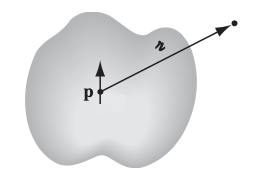
\includegraphics[width=0.4\textwidth]{./assets/Bound-charges.png}
  \end{figure}
  
\end{frame}

\begin{frame}
  \frametitle{Bound Charges}

  It is easier to work with the potentiel. 

  For a single dipole $\overrightarrow{p}$, 
  \begin{equation}
    V(\overrightarrow{r}) = \displaystyle\frac{1}{4 \pi \varepsilon_0} \displaystyle\frac{ \overrightarrow{p} . \widehat{\overrightarrow{\underline{{r}}}}}{\underline{r}^{2}}
  \end{equation}

  The total potential is the integration of each volume element, whose dipole moment $\overrightarrow{p} = \overrightarrow{P} \mathrm{d} \tau'$

  \begin{align}
    V &= \displaystyle\frac{1}{4 \pi \epsilon_0} \int_{V}^{} \displaystyle\frac{\overrightarrow{P}(\overrightarrow{r}'). \widehat{\overrightarrow{\underline{r}}}}{\underline{r}^2} \mathrm{d} \tau' \\
      &= \displaystyle\frac{1}{4 \pi \epsilon_0} \int_{V}^{} \overrightarrow{P}. \nabla ' 
  \end{align}

  
\end{frame}

% subsection The field of a polarized object (end)


\makebottom

\end{document}
